\section{Related work}

The immense number of complexities and historical artifacts that played a role in the catalysm, success and failures of the Arab Spring prohibit a full exploration of the literature here.  Instead, we here provide only a summary of some of the more widely accepted factors, and ones that readers should be aware of and keep in mind throughout the analysis. For a more detailed and accessible overview of this, we direct the reader to \citeapos{gelvin_arab_2015} recent book. We also discuss recent work utilizing social and/or news media during the Arab Spring, detailing how the methods and data used here are both similar and different.  

\subsection{Important factors}
	
A consistent take on the primary factor leading to the revolutions and their ultimate success or failure was the structure of the ruling regime\cite{bellin_reconsidering_2012,comunello_will_2012,goldstone_bringing_2013} .  \citeapos{goldstone_bringing_2013} work argues that personalist regimes were the most susceptible because their power was tied to their ability to provide the necessary economic and political incentives to their constituency.  While \cite{comunello_will_2012} notes that personalist, or as he refers to them, neopatrimonial states, had controlling arms that made it difficult to organize any sort of formal protest, a unique web of other factors led to conditions in which such formal protests could arise.

One important 



`` the relative ease with which they were overthrown depended on the availability of oil revenues and the impact of international actions.''

	1. regime structure (Goldstone)
		concurring view from \cite{bellin_reconsidering_2012,comunello_will_2012}
		
		\cite{bellin_reconsidering_2012}:
			
			the degree to which the military elite is personally invested in the regime’s survival.
	
		\cite{comunello_will_2012}
			In this environment, it is not easy to organize an uprising; in order to mobilize people and occupy squares and streets, the protestors have to challenge regimes that are particularly skilful in suppressing internal dissent

			
	2. Relationship of the military to the people and the regime
		internal factionalization within the government \cite{battera_perspectives_2014}
		
		\cite{bellin_reconsidering_2012}
			Looking at the first countries where popular protest caught fire, Tunisia and Egypt, we find four factors were essential to setting the protest in motion: long-standing grievances, an emotional trigger, a sense of impunity, and access to new social media.
				
				Emotional trigger: ordinary people take to the streets when they feel compelled by some strong emotion such as anger, fear, or euphoria. ... popular outrage in Tunisia was further stoked by a second factor as well— the decision by the regime to resort to lethal force to put down the demonstrations....Although the military ultimately refused to fire on protesters, other branches of the coercive apparatus were not so chary.
				
				Impunity: rational calculation of risk led people to join the demonstrations in large numbers once one crucial fact became clear—that the military would not shoot. ... A carnival-like atmosphere prevailed in Tahrir Square. People brought their children to witness the historic moment.
				
				Both of these are related to did the military shoot or not
	
			In every Arab country where serious protest erupted, regime survival ultimately turned on one question: would the military defect? Or, more specifically, would the military shoot the protesters or not?"
					
					In places like Tahrir Sq., where the police couldn't possibly cope w/ the number of people, it ``is sufficient to look at the character of the military and its capacity and will to repress in order to reckon the immediate chances of regime survival.''
		
		\cite{comunello_will_2012}
			Two other elements are essential to producing regime change in neopatrimonial states: first, the context involves unwilling leaders of the armed forces, too tired to defend the regime and the ‘sultan’...

			
	3. International relations (Goldstone)
		concurring view from \cite{comunello_will_2012}
			Two other elements are essential to producing regime change in neopatrimonial states: ... second, it is important that international, regional and global powers do not act to support the ‘sultan’ and prohibit the use of intolerable levels of violence against the civilian population during the revolt (Kaldor and Kostovicova 2008).
			

	4. Unified, cross-class coalition of revolutionaries (Goldstone)
		concurring view form \cite{bellin_reconsidering_2012}:
			**Using lethal force against civilians threatens to undermine the image of the military as defender of the nation, especially if the crowds are representative of the “nation” and cannot be dismissed as distinctly “other” along class, sectarian, or ethnic lines ***
			If the number of civilian challengers is small, using lethal force against them is not so problematic. But if the level of social mobilization is high, then the costs of repression will be high as well, since using lethal force against large numbers of civilians will come across as illegitimate slaughter
			
		\cite{comunello_will_2012}
			Revolts in neopatrimonial states occur at specific conjunctures, when a number of problems produce a discontent that extends to large segments of the population: the principal causes are the ineptitude of the ruling elite, difficult economic conditions and an intolerable level of corruption (Bellin 2004; Skocpol 1979). These factors allow the rebels to involve broad sections of the population in the mobilization phase, overcoming existing divisions (especially ethnic and religious discord).
		
	5. Food shortage/economic issues
		\cite{comunello_will_2012}
			The direct causes that more often trigger the urban uprisings are of two types – related either to food shortages (shortage of food itself, distribution problems or high food prices) or unemployment – or to a combination of these two factors. The first phase of the social uprisings in Egypt and Tunisia can be directly linked to precisely these two factors (Goldstone 2011).

	6. The existence of infrastructure that supported new media 
		
	\cite{bellin_reconsidering_2012}
		**none of the four factors identified as important in mobilizing protest in Egypt and Tunisia is either necessary or sufficient to explain the incidence of mass protests witnessed elsewhere during the Arab Spring. ... the cause, then, is diffusion.  David Patel, Valerie Bunce, and Sharon Wochick identify two different logics: (1) the logic of deliberate diffusion, carried out via the conscious sharing of tactics and frames by activists who are linked by networks that may be transnational; and (2) the logic of demonstration effect (that is, “the power of precedent”).**

			many political phenomena, including protest, democratization, and revolution, violate one of the fundamental assumptions of social science theorizing (including statistical analysis), namely, “the independence of cases. This seriously challenges any ambition to build predictive hypotheses rooted solely in the analysis of the causal processes governing first cases. Timing matters.

			confirms the importance of shared culture, history, and identity to explaining key political phenomena such as protest and social mobilization...it is cultural and historical proximity, not geographic vicinity, which is key to emulation	
			
		 The failure of protest to snowball in Saudi Arabia, Morocco, Algeria, and Jordan is attributable to a variety of factors, including the effective cooptation of the citizenry via the regime’s generous distribution of “buy-outs” (Saudi Arabia), societal exhaustion from prolonged civil war and the subsequent desire for calm (Algeria), and the successful division and cooptation of opposition elites topped off by the protective logic of monarchy (Morocco and Jordan). Insight into these strategies is provided by the “persistence of authoritarianism” literature cited above.
		
	\cite{comunello_will_2012}
		urban uprisings are controlled by educated individuals, often long-time residents of the city, well rooted in the metropolitan social environment (Gugler 1982).
		
	\cite{dewey_impact_2012}
	
		stagnant growth (with exceptions of Qatar and the UAE), high inflation, rising unemployment, and heavy government subsidies.
		
		Between 1950 and 2010, nearly every country in the MENA region experienced a noticeable decline in infant mortality rates in conjunction with rising fertility rates. The result has been a number of populations with disproportionately large numbers of youth. youth were enrolling in higher education, particularly at the university level. College enrollment tripled in Tunisia, quadrupled in Egypt and grew tenfold in Libya. However, the absolute increase in wealth and number of jobs failed to keep up
		
		Inflation, in particular rising food prices, also catalyzed discontent in a number of countries. By January 2011, year-on-year inflation had reached more than 6 percent in Jordan, bringing thousands into the streets to demand lower prices


\subsection{The role of new media}

	\citep{comunello_will_2012} Give an overview of early work on social media and the arab spring (pg. 461-462) ... A good review of early work, as it takes a look at how, across 8 different things, the technological determinists and the techno-realists differ on whether or not SM was useful. 
		
		Following Jenkins, contemporary society is characterized by what can be defined as convergence culture: a culture ‘where old and new media collide, where grassroots and corporate media intersect, where the power of the media producer and the power of the media consumer interact in unpredictable ways’ (Jenkins 2006, 259–60). In such a context, separating what users do with one medium from what they do with other media would be misleading: even so-called ‘old’ and ‘new’ media create a continuum, and users are constantly shifting from one platform to another.
		
		Eight dimensions of social media, where "techno-realists" and digital evangilists differ in their opinions
		(1) Ideology and planning
		2) training and tactics
		3) Communications
		4) Deployment and rapid response
		5)Costs
		6) Flexibility
		7) Resilience
		8) Propaganda/media diplomacy
		
		The Internet – and especially social media – does not determine the shift from communities to networks: rather it enables it, and makes the networked structure of society more visible, while empowering networked individuals (Rainie and Wellman 2012).
	
	
	\cite{bellin_reconsidering_2012}
		Social media (Facebook, Twitter, YouTube, cell phones with video feed capacity) and satellite television (al-Jazeera, al-Arabiya) together enabled the mobilization of collective action in ways that had been heretofore impossible in repressive settings...social media provided the means for coordinating and synchronizing thousands of people, making mass gatherings possible even in the absence of formal organizational infrastructure (something the regime would have worked hard to decimate). And when social media failed (for example, when the Egyptian regime temporarily shut down the internet), satellite television filled in the gap—with programming on al-Jazeera providing real-time coverage of events and alerting people to the location and tactics of the next protest....The past failure of social media to deliver crowds of protesters to the Kefaya movement in Egypt shows that the social media’s contribution is permissive, not deterministic ... In addition, authoritarian regimes can use this same social media to detect, monitor, divide, and rule opposition forces, illustrating its capacity to abet authoritarianism’s resilience as much as undermine it.
	
	\citep{wolfsfeld_social_2013}
		a significant increase in the use of the new media is much more likely to follow a significant amount of protest activity than to precede it. 
	
	\citep{hussein_what_2013}
	
		Digital media had a causal role in the Arab Spring by providing the very infrastructure that created deep communication ties and organizational capacity in groups of activists before the major protests took place
		
		digital technologies (may) provide the entry points for young activists to explore democratic alternatives, an action landscape such as cyberspace that allows for political discourse and even direct interventions with state policy, and coordinating mechanisms that support synchronized social movements through marches, protests, and other forms of collective action (Kirsh 2001; Warschauer, El Said, and Zohry 2002; Abdulla 2005, 2007; Shapiro 2009).
		
		Second, widespread use of mobile phone technologies was less important for the success of social movements than Internet use. However, the latter does appear as a key ingredient in two causal recipes. Therefore, having a mobile-enabled population is useful, particularly when protests have been ignited. But more than access to mobile technologies, having a long-term Internet-enabled civil society appears in all recipes.
		
		Digital media had a causal role in the
		Arab Spring by providing the very infrastructure that created deep communication
		ties and organizational capacity in groups of activists before the major protests
		took plac
		
	(hatem) 
	
	
		Things that twitter was used for:
		    Symbolic language (majority)
			meet here ... (minority)
		    documenting repression... (minority)
		Important to note that people in Egypt knew something was going to happen weeks before the 25th ... something in Cairo is gonna happen 
	
	\cite{dewey_impact_2012}
		Internet communities serve similar functions as civil society groups, particularly in countries where government repression prohibits the meeting of certain political groups.
		
		Social media increased international attention to local events in MENA by facilitating reporting from places to which traditional media has limited access
		
		Governments increasingly use social media to repress the activities of protesters and stymie democratic movements.
		
		On January 18, 2011, graduate student Asmaa Mahfouz posted a video to both Facebook and YouTube in which she called for her fellow Egyptians to participate in protests against the government. Around this time, a prominent Egyptian youth group, the April 6 Movement, contacted the then-anonymous administrator of “We Are All Khaled Saeed” asking for “marketing help” with a campaign—protests on January 25th, which would mark the official beginning of the Egypt uprisings.
		 
		
		Yemen has the lowest levels of Internet penetration in the entire MENA region, at 1.8 percent of the population
		
	\todoKenny{summarise and integrate \citep{lotan_revolutions_2011,papacharissi_affective_2012,bruns_arab_2013,hussain_what_2013,weber_secular_2013,borge-holthoefer_content_2014,siegel_tweeting_2014}}
	
	
	
	





\subsection{The role of the news media}

(hatem)

Difference between really biased newspapers ... who said nothing was really happening ... and the international news who could cover it reasonably

Egyptians relied heavily on rumors ... when you have a situation where everyone knows the news is propaganda .. you rely on rumors more  

    Also when the media is obviously lying ... I'm looking at this streety as its being recorded ... the typical egyptian deligimizes the news

	they also get a lot of international news from satellite TV ... 

\cite{hussain_what_2013}
 international news organizations played in giving them the global exposure
to help stave off overtly violent reactions from security forces.


\citep{goldstone_cross-class_2011}

The impact
of public media in favor of the protestors is also greater if media representation shows
protestors as representative of the whole society, rather than as one particular group
seeking partisan advantages for itself.
For these reasons, virtually all successful revolutions

\citep{goldstone_bringing_2013}

A peripheral
counting of media use and digital diffusion levels reveals that the countries
experiencing the most dramatic changes had low overall percentages of social
media use (Mourtada and Salem 2011). But limiting the analysis to aggregate
indicators precludes the possibility of telling a more complex, causal story. Moreover,
if there is anything to the analytical frame of networks, the use of important
media by a few important nodes of users could be exceptionally
consequential. This is why, to unpack the complexities of the Arab Spring, we
must employ analytic approaches that make possible the examination of complex
social systems that constitute the overall aggregate of state-based cases.




\subsection{\cite{goldstone_bringing_2013}}

    \begin{figure}[h]
        \centering
        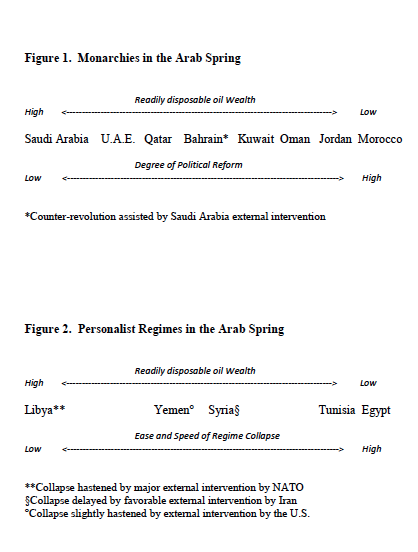
\includegraphics[width=.8\textwidth]{goldstone_2013_ssrn.png}
        \caption{\cite{goldstone_bringing_2013}}
        \label{fig:init_res}
    \end{figure}  

In Tunisia, Egypt, and Yemen seemingly invulnerable autocrats who had ruled for decades surrendered power, stepping down or fleeing in the face of mounting nation-wide popular protests. 

In Libya and Syria similarly autocratic leaders instead mobilized for war and undertook an all-out military assault on their opponents; Libya’s failed but Syria’s regime has so far succeeded in holding on to power. 

In contrast, in Algeria, Iraq, Saudi Arabia and Bahrain protests fizzled or were quickly snuffled out. 

And in Morocco, Oman, Kuwait and Jordan monarchs turned to varying degrees of constitutional reform and working with elected parliaments; in these cases reforms appear to have brought peace by deflecting demands for revolt or revolution.

Three factors of regimes that indicate how they faired:
-personalist regimes (where a single individual – who may have begun as an elected leader, or head of a military or even party regime – takes control of the national government) are particularly vulnerable to revolutionary collapse in the event of widespread popular uprising
    -monarchies () were much more stable
    
    parties are used as vehicles to push specific people through 
    
    -Personalist regimes include the regimes of Saleh in Yemen, Ghaddafi in Libya, Assad in Syria, Ben Ali in Tunisia, and Mubarak in Egypt
    -Libya is the major outlier among the personalist regimes, with vast oil revenues forming the base of the economy and providing the regime with substantial resources.
    
-a number of regimes in the region rule major oil and gas producing states. As Michael Ross (2012) has argued, states that control revenues that are easily and secretly controlled, that do not require taxation, and that are large enough to give the state the ability to maintain a large cadre of elite supporters, institutions, and popular largesse have exceptional resilience against popular demands.
    -The oil-poor states (Morocco and Jordan) went the furthest in their reforms; the oil-rich states (Oman, Kuwait, Saudi Arabia) did the least
    
-a state’s position in the international states-system has major consequences for the possibilities of change.
    - Bahrain faced perhaps the most massive protests ever seen in an authoritarian regime, in proportion to its population. However, it received help from Saudi Arabia.

In sum, the single best key to where regimes in MENA have been overturned or faced massive rebellions is where personalist regimes have arisen. In contrast to the monarchies, which all have either survived with reforms or even become counter-revolutionary, the personalist regimes have all crumbled – with the exception of Syria, which is slowly succumbing to civil war and survives in large part because of a favorable balance of external intervention.
Among these regimes, the relative ease with which they were overthrown depended on the availability of oil revenues and the impact of international actions.

It has seemed odd to many that the Arab states not yet mentioned – Lebanon, the Palestinian Authority, Iraq, and Algeria – were hardly touched by the wave of protests that erupted in the Arab Spring.

This too can be explained by a focus on the state, rather than on the structural or populist reasons for protest. The countries where the Arab Spring had its impact were monarchies and personalist regimes

Egypt and Tunisia changed their regimes with relatively little violence. Yet their change has not gone as smoothly as hoped.

Yemen has had a relatively peaceful change of regime, but it has not had peace

The vast majority of revolutionary transitions took 5 years or more, with a median of 8 years

\todoMatt{(further) summarise and integrate \citep{goldstone_cross-class_2011,goldstone_bringing_2013} into these three sections}

\todoKenny{ summarise and integrate \citep{hussein_what_2013}}


